\documentclass{article}

\usepackage{maplestd2e}
\usepackage{amssymb}
\usepackage{graphicx}
\usepackage{multicol}

\begin{document}

\bibliographystyle{ieeetr}

\begin{titlepage}
   \begin{center}
       \vspace*{1cm}

       \textbf{Security and Applications of the Blum Blum Shub Pseudo Random Number Generator}

       \vspace{0.5cm}
        To what extent do the properties of Blum Primes allow for the cryptographic security of Blum Blum Shub Pseudo Random Number Generator?
            
       \vspace{1.5cm}

       \textbf{Math}

       \vfill
            
       \vspace{0.8cm}
     
    3980 Words       
       
            
   \end{center}
\end{titlepage}

\tableofcontents
\newpage

\section{Introduction}

This essay seeks to answer \textbf{to what extent the properties of Blum Primes allow for the cryptographic security of Blum Blum Shub Pseudo Random Number Generator?} This will be explored through mathematical proof of some of the properties that allow for cryptographic security and an exploration of some the applications to the Blum Blum Shub generator. The applications of secure cryptography are vitally important as computers require the ability to transmit and store data securely. To ensure the security of encryption, cryptography relies on variety of mathematical principles. Random numbers are highly valuable in encryption for their unpredictability from attackers which allows them to be used as keys in encryption procedures, one time tokens and other important information such as password salts \cite{design2010}. A problem arises however due to the deterministic nature of computers as they can not generate numbers that are unconditionally unguessable to an adversary with unlimited computing resources \cite{design2010} \cite{Blum1986}. Sources of these include real world phenomena such as the measured radioactive decay of a radioactive source \cite{design2010}. This is where pseudo random numbers and pseudo random number generators are important. Pseudo random numbers are numbers that appear random to statistical random number tests but are generated from a deterministic pseudo random number generator algorithm \cite{Blum1986} \cite{design2010}. This poses its own problem of being predicable with knowledge of the seed value used to generate the numbers or with enough knowledge of the generator and sequentially generated numbers. The solution to this problem are cryptographically secure pseudo random number generators (CSPRNG), these meet the criteria of being polynomial time unpredictable to the right and to the left \cite{Blum1986}. This criteria allows for the generator to provide sequences of adequate quality for cryptography that are resilient to attacks by an attacker with reasonably limited computing power \cite{Blum1986}. The Blum Blum Shub generator is a CSPRNG which derives its security from the computational difficulty of finding the solution to the quadratic residuosity problem as it is akin to the computational difficulty of prime factorization \cite{Blum1986}. The exploration will focus on the link between the Blum Blum Shub generator and quadratic residues and how the computational difficulty of prime factorization provides security. Both experimental techniques and mathematical proofs will be employed to demonstrate and prove the security of BBS generator and its limitations. The combination of these techniques is important as the mathematical proofs prove the properties that allow for security and experimental testing can demonstrate both the real world strengths and weaknesses of the system. This is important as cryptographic applications are crucially important to modern computers.

\section{Definitions}

\subsection{Quadratic Residues}

In order to explore the security of the Blum Blum Shub (BBS) generator there are some preliminary definitions that must be made. The first is the definition of a quadratic residues and quadratic non-residues which are part of the base to the building of the BBS generator. A non-zero number $a$ is a quadratic residue modulo $p$ if it is congruent to a square modulo $p$ this can be written as $x^2 \equiv a \pmod{p}$ \cite{Silverman2006}. A number $a$ that is not congruent to a square modulo $p$ is considered a quadratic non residue modulo $p$ which can be written as $x^2 \not\equiv a \pmod{p}$ \cite{Silverman2006}. The solutions of $x$ for a quadratic residue modulo $p$, $a$, are considered the square roots of $a$ modulo $p$. The terms quadratic residue and quadratic non-residue can be abbreviated to QR and NR respectively.

\subsection{BBS Generator}

With the definition of QRs and NRs established the definition of the BBS generator can be defined by letting $n$ be a Blum integer and $p$ and $q$ be distinct Blum primes. The terms, Blum integer and Blum prime were coined from the creation of the BBS generator as they are the specific primes and integer that allow BBS to achieve cryptographic security. A Blum integer is defined as the product of two distinct Blum primes. A Blum prime is an odd prime $p$ where $p \equiv 3 \pmod{4}$ \cite{Pardo2012}. Thus $n = p \times q$ where $p \equiv q \equiv 3 \pmod{4}$ and $p \not= q$. Next let the set $\mathbb{Z}_n^*$ be the set of integers co-prime to $N$ thus $\mathbb{Z}_n^* = \{ x \in \mathbb{Z}| 0 < x < n, \mathit{gcd}(x,n) = 1 \}$. Let $Q_n$ be the set of all quadratic residues modulo $n$ for the terms in $\mathbb{Z}_n^*$ thus the set $Q_n$ can be created b y mapping the function $x \to x^2 \bmod n$ over $\mathbb{Z}_n^*$. With these background definitions the BBS generator can be defined in the terms of the one way function

$x_{i+1} = x_i^2 \bmod n$

Where $n$ is the Blum integer and $x_i \in Q_n$. To create a pseudo random sequence of bits each of the generated numbers either has a parity bit extracted or the least significant bit extracted.

One of the most important properties that is brought to the BBS generators by Blum primes is that each quadratic residue modulo $n$ has exactly one root that is also a quadratic residue modulo $n$ \cite{Blum1986}. This property leads to the security and unpredictability of the sequences produced by the BBS generator as it links the difficulty of predicting the next bit in the sequence to that of quadratic residousity problem \cite{Blum1986}. The proof for this fact will be explored as it relates to the use of primes. This requires the initial definition of other information.

\subsection{Legendre Symbol}

The first of this information is the Legendre symbol. It is a piecewise function of an integer, $a$ and a prime, $p$ \cite{Silverman2006}. It is defined as

$$
\left(\frac{a}{p}\right) = \left\{
                        \begin{array}{cl}  
                            1 & \mbox{if $a$ is a QR modulo $p$ and } a \not\equiv 0 \pmod{p} \\
                            -1 & \mbox{if $a$ is a NR modulo $p$} \\
                            0 & \mbox{if } a \equiv 0 \pmod{p}
                        \end{array}
                    \right.
$$

An important property of Legendre symbols is their ability to be computed using Euler's criterion  \cite{Silverman2006}. This is

$a^{(p-1)/2} \equiv \left(\frac{a}{p}\right) \pmod{p}$

A worked example of the computation of a legendre symbol is that of the integer $2$ and prime $7$.

$$
\begin{array}{l}
\left(\frac{2}{7}\right) \equiv 2^{(7-1)/2} \pmod{7} \\
\left(\frac{2}{7}\right) \equiv 2^3 \pmod{7} \\
\left(\frac{2}{7}\right) \equiv 8 \pmod{7} \\
\left(\frac{2}{7}\right) \equiv 1 \pmod{7} 
\end{array}
$$

Thus $2$ is a QR modulo $7$. This can be confirmed by the computation of $3^2 \equiv 9 \equiv 2 \pmod {7}$ where $2$ is indeed a QR modulo $7$.

\subsection{Jacobi Symbol}

The Jacobi symbol is also important and takes a similar form of $\left(\frac{a}{n}\right)$ where $a$ is an integer and $n$ is a positive odd integer \cite{Ikenaga2019}. The integer $n$ can be described as the product of its prime factors $q_1, q_2, ... q_k$. Which allows for the definition of a Jacobi symbol which is the product of the Legendre symbols of $a$ and the prime factors of $n$ \cite{Ikenaga2019}. 

$\left(\frac{a}{n}\right) = \left(\frac{a}{q_1}\right)\left(\frac{a}{q_2}\right)...\left(\frac{a}{q_k}\right)$

Like the Legendre symbol if $a$ is a quadratic residue modulo $n$ the Jacobi symbol will have the value of $1$ however the converse is not true \cite{Ikenaga2019}. A Jacobi symbol of $1$ does not indicate that $a$ is a quadratic residue modulo $n$. A worked example of this is the Jacobi symbol of 2 and 15 where 2 is an NR of 15.

\begin{center}
$$
\begin{array}{ll}
\left(\frac{2}{15}\right) = \left(\frac{2}{3}\right) \left(\frac{2}{5}\right) \\
\left(\frac{2}{3}\right) \equiv 2^{(3-1)/2} \pmod{3} & \left(\frac{2}{5}\right) \equiv 2^{(5-1)/2} \pmod{5} \\
\left(\frac{2}{3}\right) \equiv 2^1 \pmod{3} & \left(\frac{2}{5}\right) \equiv 2^2 \pmod{5} \\
\left(\frac{2}{3}\right) \equiv 2 \pmod{3} & \left(\frac{2}{5}\right) \equiv 4 \pmod{5} \\
\left(\frac{2}{3}\right) \equiv -1 \pmod{3} & \left(\frac{2}{5}\right) \equiv -1 \pmod{5} \\
\left(\frac{2}{15}\right) = (-1) (-1) = 1
\end{array}
$$
\end{center}

As observed in the example the Jacobi symbol of 2 and 15 is 1 despite 2 being a NR for all of 15, 3, and 5.

\subsection{Quadratic residuosity problem}

The quadratic residuosity problem is the problem of finding out whether an integer, $a$ is a quadratic residue modulo a number $n$, where $n$ is the product of two distinct unknown odd primes $p$ and $q$ and $\left(\frac{a}{n}\right)=1$ \cite{Hittmeir2018}. This is a problem as a Jacobi symbol equal to $1$ does not necessitate that $a$ is a quadratic residue modulo $n$. The solution to the problem is to compute the Legendre symbols $a$ with respect to $p$ and $q$ because if $\left(\frac{a}{p}\right)=\left(\frac{a}{q}\right)=1$ then this shows that $a$ is QR modulo $n$ \cite{Hittmeir2018}. The computational difficultly of this problem arises from the fact that the prime factorization of integers is computationally difficult and requires an unreasonably large amount of computational resources for an attacker.

\section{Proofs}

\subsection{$-1$ is an NR modulo a Blum prime}

For a Blum prime, $p$, then $-1$ is an NR. This can be shown from Euler's criterion since $\frac{p-1}{2}$ is always odd \cite{Fischer2017}. Then the Legendre symbol of $\left(\frac{a}{p}\right)=-1$ as $\left(\frac{a}{p}\right) \equiv -1^{(p-1)/2} \equiv -1 \bmod p$ which means that $-1$ is indeed an NR modulo $p$ \cite{Fischer2017}. It follows that $-1$ is also an NR modulo a Blum integer, $n$ however in this case the Jacobi symbol of $\left(\frac{-1}{n}\right)$ is equal to $1$ as:

$\left(\frac{-1}{n}\right)=\left(\frac{-1}{p}\right) \left(\frac{-1}{q}\right)=(-1)(-1)=1$

\subsection{Exactly one QR modulo a Blum prime}

If $p$ is a Blum prime and $\pm b$ are the two square roots of $a$, a quadratic residue modulo $p$, it can be shown that exactly one of $b$ and $-b$ is also a quadratic residue modulo $p$ \cite{Fischer2017}. This can be expressed in terms of the Legendre Symbols for $b$ and $-b$ which gives $\left(\frac{-b}{p}\right) \not= \left(\frac{b}{p}\right)$. Which can then be represented in terms of Euler's criterion to give, $(-b)^{(p-1)/2} \not= (b)^{(p-1)/2}$ \cite{Fischer2017}. This equation can be proved since

$(-b)^{(p-1)/2}=(-1)^{(p-1)/2} b^{(p-1)/2}=(-1) b^{(p-1)/2}$

As both $\left(\frac{b}{p}\right)$ and $\left(\frac{-b}{p}\right)$ are either $-1$ or $1$, it follows from the definition of the Legendre Symbol that $(-b)^{(p-1)/2}$ and $b^{(p-1)/2}$ are either $1$ or $-1$. From Euler's criterion it follows that one of $b$ and $-b$ is a quadratic residue modulo $p$ and the other is not \cite{Fischer2017}.

\subsection{Find two roots of a QR}

It can be shown that there the two roots of a QR, $a$ modulo a Blum prime $p$, can be found as $\pm a^{(p+1)/4} \pmod{p}$ \cite{Mora2013}. This definition of roots allows for the quick computation of roots modulo Blum primes due to them satisfying $p \equiv 3 \pmod{4}$ \cite{Blum1986}. This is useful in different applications of the BBS generator. This property can be proved by working backwards.

$$
\begin{array}{l}
\pm (a^{(p+1)/4})^2 \\
= a^{(p+1)/2} \\
= a^{(p-1)/2}  a \\
= \left(\frac{a}{p}\right)  a \mbox{ from the definition of the Legendre symbol} \\
= a \because \mbox{ $a$ is QR modulo $p$}
\end{array}
$$

\subsection{One root of a QR modulo a Blum integer is a QR}

With these things defined the property that exactly one of the roots of a QR modulo a Blum integer is also a QR modulo the Blum integer can be shown. As a Blum integer is the product of two Blum primes the roots of a QR modulo the Blum integer are determined by the two Blum primes. To start let $a$ be a QR modulo a Blum integer, $n$, which is the product of two Blum primes $p$ and $q$. Additionally let the integer $b_p$ be an integer such that $-\frac{p}{2} < b_p < \frac{p}{2}$ and $a \equiv b_p^2 \pmod{p}$ and similarly let $b_q$ be an integer such that $-\frac{q}{2} < b_q < \frac{q}{2}$ and $a \equiv b_q^2 \pmod{q}$ \cite{Mora2013}. Thus the four roots modulo $n$ can be defined in terms of these roots modulo $q$ and $p$ \cite{Mora2013}. These are:

$$
\begin{array}{l}
x_1, -\frac{n}{2} < x_1 < \frac{n}{2} \mbox{ s.t. } x_1 \equiv b_p \pmod{p}, x_1 \equiv b_q \pmod{q} \\
x_2, -\frac{n}{2} < x_2 < \frac{n}{2} \mbox{ s.t. } x_2 \equiv -b_p \pmod{p}, x_2 \equiv -b_q \pmod{q} \\
x_3, -\frac{n}{2} < x_3 < \frac{n}{2} \mbox{ s.t. } x_3 \equiv b_p \pmod{p}, x_3 \equiv -b_q \pmod{q} \\
x_4, -\frac{n}{2} < x_4 < \frac{n}{2} \mbox{ s.t. } x_4 \equiv -b_p \pmod{p}, x_4 \equiv b_q \pmod{q}
\end{array}
$$

A worked example of this is the primes $p$ and $q$ of $7$ and $11$ respectively and the Blum integer, $n$ of 77. The QR of $71$ and its roots of $15, 29, 48$ and $62$ will be used to show this property. First $b_p$ and $b_q$ can be found using the formula for the roots of Quadratic residues from Section 3.3.

$$
\begin{array}{l}
b_p = \pm 71^{(7+1)/4} \bmod 7 \\
b_p = \pm 1 \bmod 7 \\
b_q = \pm 71^{(11+1)/4} \bmod 11 \\
b_q = \pm 4 \\
\end{array}
$$

Thus the relationship between $b_p$, $b_q$ and the four roots can be shown.

$$
\begin{array}{llll}
x_1 \equiv b_p \bmod p & x_2 \equiv -b_p \bmod p & x_3 \equiv b_p \bmod p & x_4 \equiv -b_p \bmod p \\
15 \equiv 1 \bmod 7 & 62 \equiv -1 \bmod 7 & 29 \equiv 1 \bmod 7 & 48 \equiv -1 \bmod 7 \\
x_1 \equiv b_q \bmod q & x_2 \equiv -b_q \bmod q & x_3 \equiv -b_q \bmod q & x_4 \equiv b_q \bmod q \\
15 \equiv 4 \bmod 11 & 62 \equiv 7 \bmod 11 & 29 \equiv -4 \bmod 11 & 48 \equiv 4 \bmod 11  
\end{array}
$$

An important note about the four roots is that $x_1 = -x_2 \pmod{n}$ while $x_1 \not= \pm x_3 \pmod{n}$ \cite{Mora2013}. From this $x_1$ and $x_2$ can be represented as $x$ and $-x$ respectively and $x_3$ and $x_4$ can be represented as $y$ and $-y$ respectively \cite{Mora2013}. These conditions for the roots of the quadratic residue give similar notions for the Legendre symbols of the roots in relation to $p$ and $q$ and allow a pattern to be seen in regards to the Jacobi symbols of the roots \cite{Mora2013}. This is:

$$
\begin{array}{l}
\left(\frac{x}{p}\right) = \left(\frac{b_p}{p}\right) = 1, \left(\frac{x}{q}\right) = \left(\frac{b_q}{q}\right) = 1, \left(\frac{x}{n}\right) = \left(\frac{x}{p}\right)  \left(\frac{x}{q}\right) = 1 \\
\left(\frac{-x}{p}\right) = \left(\frac{-b_q}{q}\right) = -1, \left(\frac{-x}{q}\right) = \left(\frac{-b_q}{q}\right) = -1, \left(\frac{-x}{n}\right) = \left(\frac{-x}{p}\right)  \left(\frac{-x}{q}\right) = 1 \\
\left(\frac{y}{p}\right) = \left(\frac{b_p}{p}\right) = 1, \left(\frac{y}{q}\right) = \left(\frac{-b_q}{q}\right) = -1, \left(\frac{y}{n}\right) = \left(\frac{y}{p}\right)  \left(\frac{y}{q}\right) = -1 \\
\left(\frac{-y}{p}\right) = \left(\frac{-b_p}{p}\right) = -1, \left(\frac{-y}{q}\right) = \left(\frac{b_q}{q}\right) = 1, \left(\frac{-y}{n}\right) = \left(\frac{-y}{p}\right)  \left(\frac{-y}{q}\right) = -1 \\
\end{array}
$$

From this it can be seen that $\left(\frac{\pm x}{n}\right)= -\left(\frac{\pm y}{n}\right)$ \cite{Mora2013}. It is then important to further investigate the roots that have a Jacobi symbol of $1$ in regards to $n$ as they are the only roots that could possibly also be a quadratic residue modulo $n$. These roots are indistinguishable by Jacobi symbol however one will aso be quadratic residue modulo $n$ namely the root, $x$, which is congruent to a quadratic residue modulo p and modulo q thus this root satisfies $\left(\frac{x}{p}\right) = \left(\frac{x}{q}\right) = 1$ \cite{Mora2013}. It is valuable to have a way to easily distinguish this root from the other root with a Jacobi Symbol of $1$. This can be can be partially found through an initial assumption and a proof through Euler's criterion. The assumption is that given $\left(\frac{x}{p}\right) = \left(\frac{x}{q}\right) = 1$ then it implies that $x^{((p-1)(q-1))/4} \equiv 1 \pmod{n}$ \cite{Mora2013}. This can be proved by looking at the statement with respect to both $p$ and $q$ as they are the prime factors of $n$, where there is, 

$$
\begin{array}{l}
    x^{((p-1)(q-1))/4} \pmod{p} \\
    = (x^{(p-1)/2})^{(q-1)/2} \pmod{p} \\
    \equiv \left(\frac{x}{p}\right)^{(q-1)/2} \pmod{p} \mbox{  from the definition of the Legendre symbol} \\
    = 1^{(q-1)/2} \pmod{p}\\
    = 1 \pmod{p}
\end{array}
$$

and similarly

$$
\begin{array}{l}
    x^{((p-1)(q-1))/4} \pmod{q} \\
    = (x^{(q-1)/2})^{(p-1)/2} \pmod{q} \\
    \equiv \left(\frac{x}{q}\right)^{(p-1)/2} \pmod{q} \mbox{  from the definition of the Legendre symbol} \\
    = 1^{(p-1)/2} \pmod{q}\\
    = 1 \pmod{q}
\end{array}
$$

whence $x^{((p-1)(q-1))/4} \equiv 1 \pmod{n}$ \cite{Mora2013}. It can be shown that the converse of this is true, that if a root fulfills the criteria $x^{((p-1)(q-1))/4} \equiv 1 \pmod{n}$ it implies that the root satisfies $\left(\frac{x}{p}\right) = \left(\frac{x}{q}\right) = 1$ \cite{Mora2013}. This can be done starting that by assumption $x^{((p-1)(q-1))/4} \equiv 1 \pmod{p}$ and $x^{((p-1)(q-1))/4} \equiv 1 \pmod{q}$ \cite{Mora2013}. Since $n$ is a Blum integer, both $\frac{p-1}{2}$ and $\frac{q-1}{2}$ are odd and so is $\frac{(p-1)(q-1)}{4}$ therefore 

$\left(\frac{x}{p}\right) = \left(\frac{x}{p}\right)^{((p-1)(q-1))/4} = \left(\frac{x^{((p-1)(q-1)/4)}}{p}\right) = \left(\frac{1}{p}\right) = 1$

and similarly 

$\left(\frac{x}{q}\right) = \left(\frac{x}{q}\right)^{((p-1)(q-1))/4} = \left(\frac{x^{((p-1)(q-1)/4)}}{q}\right) = \left(\frac{1}{q}\right) = 1$

The other root, $-x$, that has a Jacobi symbol of $1$ and satisfies $\left(\frac{-x}{p}\right) = \left(\frac{-x}{q}\right) = -1$ has similar properties. It will satisfy $(-x)^{((p-1)*(q-1))/4} \equiv -1 \pmod{n}$ this is because $\frac{(p-1)(q-1)}{4}$ is always odd \cite{Mora2013}. This can be shown through a full proof in a similar manner to the other root $x$, where it can be verified that the root $-x$ is indeed an NR modulo $n$. This with the fact that since $\left(\frac{-x}{p}\right) = \left(\frac{-x}{q}\right) = -1$ then by Euler's Criterion,

$$
\begin{array}{l}
    (-x)^{((p-1)(q-1))/4} \pmod{p} \\
    = ((-x)^{(p-1)/2})^{(q-1)/2} \pmod{p} \\
    \equiv \left(\frac{-x}{p}\right)^{(q-1)/2} \pmod{p} \mbox{  from the definition of the Legendre symbol} \\
    = (-1)^{(q-1)/2} \pmod{p}\\
    = -1 \pmod{p}
\end{array}
$$

and similarly

$$
\begin{array}{l}
    (-x)^{((p-1)(q-1))/4} \pmod{q} \\
    = ((-x)^{(q-1)/2})^{(p-1)/2} \pmod{q} \\
    \equiv \left(\frac{-x}{q}\right)^{(p-1)/2} \pmod{q} \mbox{  from the definition of the Legendre symbol} \\
    = (-1)^{(p-1)/2} \pmod{q}\\
    = -1 \pmod{q}
\end{array}
$$

whence $(-x)^{((p-1)(q-1))/4} \equiv -1 \pmod{n}$ \cite{Mora2013}. We can also similarly show the converse where if a root satisfies $(-x)^{((p-1)(q-1))/4} \equiv -1 \pmod{n}$ it implies it will also satisfy $\left(\frac{-x}{p}\right) = \left(\frac{-x}{q}\right) = -1$ \cite{Mora2013}. This can be shown with the assumption of $(-x)^{((p-1)(q-1))/4} \equiv -1 \pmod{b}$ and $(-x)^{((p-1)(q-1))/4} \equiv -1 \pmod{q}$ then since $\frac{(p-1)(q-1)}{4}$ is odd it is obtained that,

$\left(\frac{-x}{p}\right) = \left(\frac{-x}{p}\right)^{((p-1)(q-1))/4} = \left(\frac{(-x)^{((p-1)(q-1)/4)}}{p}\right) = \left(\frac{-1}{p}\right) = -1$

and similarly 

$\left(\frac{-x}{q}\right) = \left(\frac{-x}{q}\right)^{((p-1)(q-1))/4} = \left(\frac{-x^{((p-1)(q-1)/4)}}{q}\right) = \left(\frac{-1}{q}\right) = -1$

To verify that these conditions are the case for the roots of $x$ and $-x$ the numbers used previously can be used for a worked example ($p = 7, q=11, n=77, x=15, -x=62$). For the root $x$ it can be shown that $x^{((p-1)(q-1))/4} \equiv 1 \pmod{p}$ as:

$15^{((7-1)(11-1))/4} \equiv 15^15 \equiv 1 \pmod{77}$

Similarly the fact that $(-x)^{((p-1)(q-1))/4} \equiv -1 \pmod{n}$ can be shown as:

$62^{((7-1)(11-1))/4} \equiv 62^15 \equiv 76 \equiv -1 \pmod{77}$

From these proofs show the fact that one and only of the four roots of a quadratic residue modulo a Blum integer is itself a quadratic residue namely this root is the root $x$ which satisfies both of $\left(\frac{x}{n}\right) = 1$ and $x^{((p-1)(q-1))/4} \equiv 1 \pmod{n}$ \cite{Mora2013}. 

The fact that the property that exactly one quadratic root of four is also a quadratic residue modulo $n$ is present allow for the security of the Blum Blum Shub generator. This property leads to the quadratic residuosity problem always appearing if an attacker wants to work backward \cite{Blum1986}. This is the case due to the two roots that both have a Jacobi symbol of $1$ with respect to $n$ \cite{Fischer2017}. Thus if the correct root is to be found knowledge of $p$ and $q$ is required and so the attacker must factorize $n$. This will be shown by investigation to be computationally difficult with a sufficiently large $n$ and is also widely accepted fact with current technology \cite{Landquist2001} \cite{Blum1986}. This makes the generator secure to being predicted in reverse. The logic for the security forwards when the Blum Blum Shub generator has the parity of each generated term extracted is similar. It requires the assumption that the prime factorization of integers is computationally difficult. This is because if from knowledge of the seed of the generator, a random portion of the generated sequence of bits and $n$ it was possible to gain advantage in predicting the next bit there would be a fast algorithm for finding the factorization of $n$ \cite{Blum1986} \cite{Faisal2017}. Thus as prime factorization is difficult as assumed with current computers there cannot be a polynomial time algorithm to successfully predict the next bit of the Blum Blum Shub generator when the parity of each generator number is taken as a bit in the sequence \cite{Blum1986} \cite{Faisal2017}.

\section{Applications}

\subsection{Public Key Cryptography Example}

The property of being predictable backwards with knowledge of $p$ and $q$ can be exploited for use in public key cryptography. This is important to investigate as this implementation of public key encryption is similar in security to that of the widely used RSA encryption which also relies on security based on the computational difficulty of integer factorization. This is used to secure internet traffic as the information for encryption is shared publicly however the message can only be decrypted by the party with the private key. A worked example of this with Bob wanting to send Alice a secure message over public channels will be used. To begin Alice must first define her private keys, $p$ and $q$, both of which must be Blum primes. For this example the small primes of $19$ and $23$ will be used. Alice's public key is then defined as, $n=437$, the product of the private keys $p$ and $q$. Alice then shares the public key with everyone to allow people to send encrypted messages to her. In order to send the message to her Bob uses the public to generate a one time pad. This is achieved by taking a seed that is co-prime to $n$ and squaring it and taking it modulo $n$ repeating this for a specified length, $i$. For this example the seed will be $64$ and the length of the sequence will be $8$. This can be implemented with the loop given in Appendix A.1 this gives a sequence of:


$$[163, 349, 315, 26, 239, 311, 144, 197]$$

Once a series of pseudo random numbers is generated a series of pseudo random bits is created by extracting the least significant bit of each number. It is also possible to extract the parity of each of the numbers as the bit or more of the least significant bits however this example will only use one least significant bit \cite{Blum1986}. The operation for extracting the least significant bit is taking each pseudo random number modulo $2$ the implementation is given in Appendix A.2. The $x_{i+1}$ number of the $i$ length sequence is also recorded with the pad to be used by the recipient later, this gives:

$$[[1, 1, 1, 0, 1, 1, 0, 1], 353]$$

With the created pad and a message of the same length that Bob wants to send he can encrypt by using the XOR operator across the two sets of bits (equivalent to the sum of bits mod 2) \cite{Blum1986}. This encrypted message is sent with the $x_{i+1}$ number generated when creating the one time pad so that Alice can decode it later. The implementation is given in Appendix A.3. If his message is:

$$[0, 1, 0, 0, 1, 1, 1, 0]$$

then the encrypted message is:

$$[[1,0,1,0,0,0,1,1],353]$$

Once Alice receives Bob's encrypted message she must first rebuild his onetime pad. This requires the knowledge of her private keys p and q and the $X_{i+1}$ term of the sequence that Bob generated before extracting bits, using this the sequence generated by Bob can be determined in reverse \cite{Blum1986}. First using the Extended Euclidean Algorithm the variables $u,v$ which satisfy the equation $p*u+q*v=1$ are determined. The Extended Euclidean Algorithm determines the greatest common denominator of two numbers and a solution to $ax+by=gcd(x,y)$ where $x,y$ are known \cite{Silverman2006}. The implementation the Extended Euclidean Algorithm is Appendix B \cite{Brilliant2020}. This algorithm can be used to generate $u,v$ which are $-6$ and $5$ respectively. After determining u and v the roots $x_p, x_q$ that are the solutions to $x_p = \sqrt{x_{i+1}} \bmod p$ and $x_q = \sqrt{x_{i+1}} \bmod p$ where $x_{i+1}$ is Bob's term to be worked backward from and $x_p, x_q$ satisfy $\left(\frac{x_p}{p}\right) = +1$ and $\left(\frac{x_q}{q}\right) = +1$ respectively must be found. Since $p \equiv q \equiv 3 \pmod{4}$ this can be efficiently computed using the formula $x_p \equiv \pm x_{i+1}^{\frac{p+1}{4}} \bmod p$ then finding the Legendre symbol of each root \cite{Faisal2017}. Working through the math in the example this looks like:

$$
\begin{array}{ll}
x_p \equiv \pm x_{i+1}^{\frac{p+1}{4}} \bmod p & x_q \equiv \pm x_{i+1}^{\frac{p+1}{4}} \bmod q \\
x_p \equiv \pm 353^{\frac{19+1}{4}} \bmod 19 & x_q \equiv \pm 353^{\frac{23+1}{4}} \bmod 23 \\
x_p \equiv \pm 353^{5} \bmod 19 & x_q \equiv \pm 353^{6} \bmod 23 \\
x_p \equiv \pm 7 \bmod 19 & x_q \equiv \pm 13 \bmod 23 \\
\left(\frac{7}{19}\right) \equiv 7^{(19-1)/2} \bmod 19 & \left(\frac{13}{23}\right) \equiv 13^{(23-1)/2} \bmod 23 \\
\left(\frac{7}{19}\right) \equiv 1 \bmod 19 & \left(\frac{13}{23}\right) \equiv 1 \bmod 23 \\
\left(\frac{-7}{19}\right) \equiv -7^{(19-1)/2} \bmod 19 & \left(\frac{-13}{23}\right) \equiv -13^{(23-1)/2} \bmod 23 \\
\left(\frac{-7}{19}\right) \equiv -1 \bmod 19 & \left(\frac{-13}{23}\right) \equiv -1 \bmod 23 \\
\because \mbox{ } \left(\frac{7}{19} \right) = 1 & \because \left(\frac{13}{23}\right) = 1 \\
\therefore x_p = 7 & \therefore x_q = 13
\end{array}
$$

With these variables computed the term one before Bobs in the sequence, $x_N$, can be found using the equation $x_N = x_p \times q \times v+x_q \times p \times u$ \cite{Blum1986}.

$$
\begin{array}{l}
x_N = x_p \times q \times v+x_q \times p \times u \bmod N \\
x_N = 7 \times 23 \times 5+13 \times 19 \times -6 \bmod 437 \\
x_N = -667 \bmod 437 \\
x_N = 197
\end{array}
$$

This is then repeated for the length $i$ of the message to work backwards and create Bob's pad in reverse. This array is then flipped and the least significant is then extracted to recreate Bobs pad. The procedural implementation of this in Maple is Appendix C. Alice can then generate the pad:

$$[1, 1, 1, 0, 1, 1, 0, 1]$$

With Bob's pad generated Alice can then use the XOR operator with the pad and encrypted message to decrypt Bob's message giving back the message:

$$[0, 1, 0, 0, 1, 1, 1, 0]$$

This safe communication is possible due to the properties of the two Blum primes that act as Alice's private keys and their ability to work backward through the generator. If communication needed to be two way between Alice and Bob they would both need their own set of private and public keys. 

\subsection{Exploring the security of factorization}

Part of what makes the Blum Blum Shub cryptographically secure and applicable in real world applications is the computational difficulty of solving the quadratic residuosity problem due to the requirement to prime factor large integers. The security of factorization will be explored in this section to show how it currently protects messages and how it could eventually be inviable for security. This was explored experimentally by factoring Blum integers of varying lengths using the quadratic sieve algorithm and recording the CPU time required to factorize. The quadratic sieve algorithm is the second fastest factorization algorithm and the fastest for integers under 110 digits long \cite{Landquist2001}. It is thus useful in the investigation of the practical ability of an attacker to factorize $n$ and crack the Blum Blum Shub generator. The data in this investigation was collected on a laptop with a mobile Intel i7 CPU using the code provided in Appendix D. 

\begin{figure}
    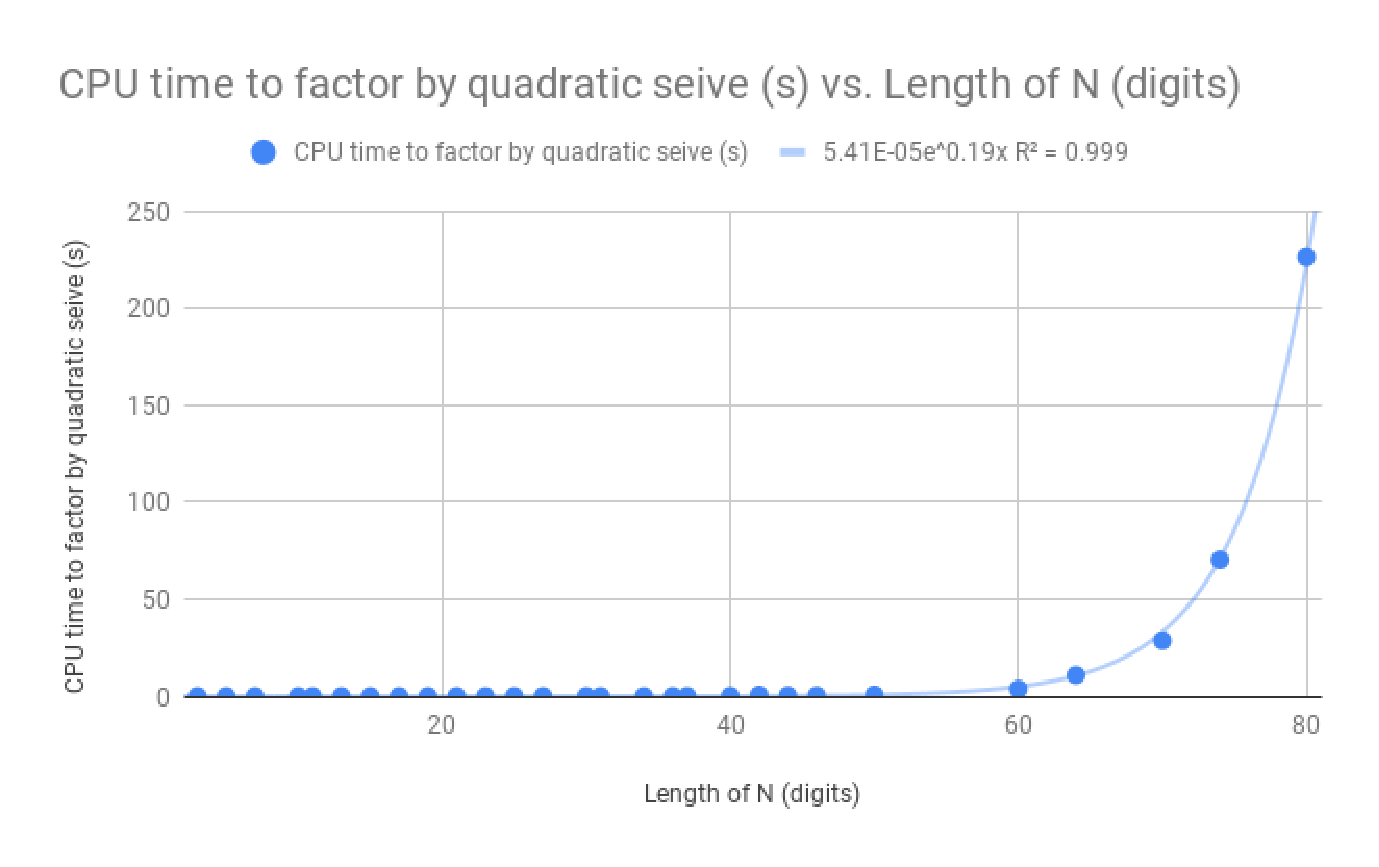
\includegraphics[scale=0.5]{graph1.eps}
    \caption{A graph of the CPU time taken to factorize Blum integers by quadratic sieve vs the length of the Blum integer}
    \label{fig:graph1}
\end{figure}

From \ref{fig:graph1} it can be seen that the CPU time taken to factorize the Blum integer increases exponentially with the length of the Blum integer. When the Blum integer is short enough it can be factored practically instantly. This very quickly changes once the integers reach approximately 70 digits as the operation begins to take significantly longer. Additionally when an integer of 100 digits in length was attempted to be factored the operation took over 10 minutes then was killed without finishing. This is mostly in line with the Big O notation of the quadratic sieve algorithm of $O(e^{\sqrt{1.125\ln(n)\ln(\ln(n))}})$ which indicates its worst case complexity with varying input length \cite{Landquist2001}. This was the case asides from the very high efficiency with short integers. Due to this high complexity of factoring, keys of 2048-bit lengths have been deemed secure by The National Institute of Stands and Technology for cryptographic use until at least 2030 \cite{Thayer2020}. This security however diminishes with improvements to processing power as they allow for larger and larger keys to be factorized breaking the security of the CSPRNG \cite{Landquist2001}. This is becoming even more of a problem due to the improvements in quantum computing which once quantum computers of approximately 1000 Qubits exist will alow for polynomial time factorization of integers \cite{Landquist2001}. This will effectively negate the security of any cryptographic systems based on the difficulty of factorization such as RSA which is typically used in public key cryptography and the Blum Blum Shub generator \cite{Landquist2001}. Since these improvements have not happened yet number generation and cryptography based on the difficulty of prime factorization is still secure however cryptographic methods must continue to evolve and improve in order stay ahead of the ability to crack them.

\subsection{Other Applications}

While the Blum Blum Shub generator is currently very secure and can theoretically be used for public key encryption it is also relatively slow and inefficient making this use case impractical in the real world as RSA is more efficient. The real world applications of the BBS generator are primarily in situations where generation rate is not critical such as producing keys in asymmetric systems such as RSA or password based key derivation where keys are generated once \cite{Vybornova2017}. The slow rate of generation (23 kb/s) the BBS generator has compared to modern symmetric block cyphers such as AES (2.5 Gb/s) and the two fish algorithm (415 Mb/s) limits its range of applications \cite{Vybornova2017}. This slow speed due to its computational complexity can be a benefit in some application where this increases the security, while making it inapplicable to others.

\section{Conclusion}

In conclusion Blum Primes are crucial to the security of the Blum Blum Shub generator due to the properties they have. Specifically they liken the difficulty of predicting the Blum Blum Shub generator in either direction to the difficulty of the quadratic residuosity problem. This makes it a requirement to be able to quickly factor large integers in order to attack the Blum Blum Shub generator. This is currently computationally difficult as it is not possible to factor integers in polynomial time. This lends the Blum Blum Shub generator to be highly secure and unpredictable. This security will not all ways be present as greater computational power will allow for the increased ability of attackers to break cryptographic systems and generators such as the BBS generator that rely on the security given by the difficultly of factorization. This threat is increasingly present with the rise of quantum computers which once sufficiently advanced will offer the ability to factorize integers in polynomial time. A development like this will render the BBS generator completely insecure and obsolete. Once this development occurs a significant rethink of cryptography will be required as the public key encryption that secures the internet will be obsolete. Constant innovation and new developments are always going to be required especially in the field of cryptography to overcome increasingly capable attackers. Overall Blum primes are the key to the security of the BBS generator and provably allow the generator to be cryptographically secure against current technology however they are limited in security by the increasing threat of greater computational power and quantum computing which can eventually render the BBS generator obsolete.

\newpage
\bibliography{ee}

\newpage
\appendix

\section{Public Key Encryption Implementation}
\subsection{BBS Generator Loop}
\begin{verbatim}
    > Bobs_Pseudo_Random_Numbers := Array(1..1, [64^2 mod n]):
    > for i from 1 to 8 - 1 do
          Bobs_Pseudo_Random_Numbers ,= Bobs_Pseudo_Random_Numbers(i)^2 mod n:
      end do:
\end{verbatim}

\subsection{Parity of Sequence Members}
\begin{verbatim}
    Bobs_Pad := [map(a -> a mod 2, convert(Bobs_Pseudo_Random_Numbers,list)),                
        Bobs_Pseudo_Random_Numbers(-1)^2 mod N];
\end{verbatim}

\subsection{Message Encryption}
\begin{verbatim}
    Bobs_Message_Encrypted := [Bobs_Pad[1] + Bobs_Message mod 2, Bobs_Pad[2]]
\end{verbatim}

\subsection{Message Decryption}
\begin{verbatim}
    Alice_Decrypted_Message := Bobs_Message_Encrypted[1] + 
        Alices_Generated_Pad mod 2;
\end{verbatim}

\section{Extended Euclidean Algorithm}

\begin{verbatim}
    Extended_Euclidean_Algorithm := proc(c, d)
       local a,b,x,y,u,v,m,n,q,r;
       a,b := c,d;
       x,y, u,v := 0, 1, 1, 0;

       while a <> 0 do
           q, r := floor(b/a), b mod a;
           m, n := x-u*q, y-v*q;
           b, a, x, y, u, v := a, r, u, v, m, n;
       end do;

       local gcd := b;
       return [x, y];
    end proc:
\end{verbatim}

\section{Recreate Pad Function}

\begin{verbatim}
    local Recreate_Pad := proc(p, q, x, length:=8)
       local u,v,xp,xq,xn,N;

       N := p*q;
       u,v := Extended_Euclidean_Algorithm(p, q)[];
       xp := select(i -> NumberTheory:-LegendreSymbol(i, p) = 1, 
        [x^(p+1)/4) mod p, -x^((p+1)/4) mod p])[];
       xq := select(i -> NumberTheory:-LegendreSymbol(i, q) = 1, 
        [x^((q+1)/4) mod q, -x^((q+1)/4) mod q])[];
       xn := xp*q*v + xq*p*u mod N;
       local result := Array(1..1, xn);

       for local h to length - 1 do
             xp := select(i -> NumberTheory:-LegendreSymbol(i, p) = 1, 
                [result(h)^((p+1)/4) mod p, -result(h)^((p+1)/4) mod p])[];
             xq := select(i -> NumberTheory:-LegendreSymbol(i, q) = 1, 
                [result(h)^((q+1)/4) mod q, -result(h)^((q+1)/4) mod q])[];
             xn := xp*q*v + xq*p*u mod N;
             result ,= xn;
       end do;

       return map(i -> i mod 2, 
        convert(ArrayTools:-FlipDimension(result, 2), ':-list'));
    end proc;
\end{verbatim}

\section{Factorization of Varying Length Blum Integers}
\begin{verbatim}
    > t := Array(1..0):
    > for pair in BlumPrimes do 
          n := mul(pair):
          n_Length := StringTools:-Length(cat("",n));
          t ,= [n_Length, [CodeTools:-CPUTime(ifactor(n))][1]];
          forget(ifactor); #clear cache for control between factorizations
      end do:
\end{verbatim}

\end{document} 
